\documentclass[11pt,a4paper]{article}

\usepackage[T1]{fontenc}
\usepackage[utf8]{inputenc}
\IfFileExists{lmodern.sty}{\usepackage{lmodern}}{}
\usepackage[margin=2.5cm]{geometry}
\usepackage{amsmath,amssymb,amsthm,bm}
\usepackage{mathtools}
\usepackage{graphicx}
\usepackage{booktabs}
\usepackage{array}
\usepackage[authoryear,round]{natbib}
\usepackage{xcolor}
\usepackage[colorlinks=true,linkcolor=blue!50!black,citecolor=blue!50!black,urlcolor=blue!50!black]{hyperref}
\usepackage{caption}
\usepackage{enumitem}

\newtheorem{proposition}{Proposition}
\newtheorem{lemma}{Lemma}
\theoremstyle{remark}
\newtheorem{remark}{Remark}

\newcommand{\vect}[1]{\bm{#1}}
\newcommand{\uv}[1]{\hat{\bm{#1}}}
\newcommand{\R}{\mathbb{R}}
\newcommand{\Sph}{\mathbb{S}^2}
\newcommand{\dd}{\,\mathrm{d}}
\newcommand{\T}{^{\mathsf T}}
\newcommand{\Req}{R_{\mathrm{eq}}}
\DeclareMathOperator{\diag}{diag}
\DeclareMathOperator{\tr}{tr}
\DeclareMathOperator*{\argmin}{arg\,min}
\DeclareMathOperator*{\argmax}{arg\,max}

\title{Bayesian convex lightcurve inversion with Laplace-marginalised shapes and nested sampling:\\
methodology and application to Rubin Observatory photometry of 2003~QN$_{21}$}
\author{Methods note accompanying the \texttt{lcinv} prototype}
\date{29 October 2026}

\begin{document}
\maketitle

\begin{abstract}
We describe a Bayesian framework for recovering the spin state and convex shape of an asteroid,
with uncertainties, from disk-integrated multi-band photometry. The forward model is the classical
Gaussian-image convex inversion of \citet{kaasalainen2001a,kaasalainen2001b} with a
Lommel--Seeliger plus Lambert scattering law, implemented in a differentiable form. Four
methodological elements distinguish the approach from the standard $\chi^2$-minimisation workflow:
(i) a white-noise ``jitter'' term that absorbs unmodelled photometric systematics;
(ii) analytic profiling of band offsets and the phase-angle slope, and Laplace marginalisation of
the shape coefficients at every spin state;
(iii) the observation that the rotational phase is a gauge freedom of a free convex shape, which
reduces the sampled space to pole longitude, pole latitude, sidereal period and jitter;
(iv) nested sampling of this four-dimensional posterior, followed by a posterior shape ensemble
obtained from Laplace draws and an exact Minkowski reconstruction posed as a convex optimisation
problem. Lightcurve-derived priors on the period and on the equatorial axis ratio are included
optionally. Diagnostics comprise injection--recovery tests, global-optimum checks of the inner
optimiser, importance re-weighting with a finer surface discretisation, registered radius-uncertainty
maps, and a rotational-stability test based on the inertia tensor. We apply the method to 334
$gri$ measurements of 2003~QN$_{21}$ obtained by the Rubin Observatory over five nights. The
sidereal period is $3.24828^{+0.00025}_{-0.00032}$\,h. The pole posterior is bimodal, with the
mirror solutions $(\lambda,\beta)\approx(67^\circ,+71^\circ)$ and $(244^\circ,-73^\circ)$, each
$\approx15^\circ$ wide at 68\% credibility. The stability diagnostic shows that the posterior
shapes do not rotate about their axis of maximum inertia, which identifies a stronger physical
shape constraint as the main required improvement.
\end{abstract}

\tableofcontents

%==========================================================================================
\section{Introduction}
\label{sec:intro}

Disk-integrated photometry is by far the most abundant source of information on asteroid shapes and
spins. The modern inversion problem was formulated by \citet{kaasalainen1992} and solved in practical
form by \citet{kaasalainen2001a} and \citet{kaasalainen2001b}. They showed that a convex model,
parametrised by its Gaussian image and constrained by a smooth scattering law, reproduces dense
lightcurves to the noise level and yields a unique solution, up to known symmetries, when the viewing
geometries are sufficiently diverse. The Minkowski reconstruction of the polyhedron from its facet
areas was treated by \citet{little1983} and \citet{lamberg1993}. Sparse and dense data were combined
by \citet{durech2009}, and the resulting models are collected in DAMIT \citep{durech2010}. Uniqueness
and the fundamental ambiguities of the lightcurve operator are discussed by \citet{kaasalainen2006}.

Uncertainty quantification in this field has evolved from $\chi^2$ thresholds
\citep[e.g.][]{durech2018} through bootstrap ensembles to fully Bayesian treatments, notably the
virtual-observation Markov chain Monte Carlo approach of \citet{muinonen2020}. Non-convex and
multi-data-type extensions include ADAM \citep{viikinkoski2015} and SAGE \citep{bartczak2018}.

Survey photometry from the Vera C.\ Rubin Observatory \citep{ivezic2019} motivates a pipeline that is
automatic and statistically explicit. It must also be honest about weakly constrained cases, such as a
single apparition observed over a few nights. This note documents the mathematics of such a pipeline:
\begin{itemize}[nosep]
\item the photometric reduction and ephemeris geometry (\S\ref{sec:geometry});
\item the period search and lightcurve-derived priors (\S\ref{sec:period});
\item the forward model (\S\ref{sec:model}) and the gauge freedom of the rotational phase
  (\S\ref{sec:gauge});
\item shape priors and axis-ratio functionals (\S\ref{sec:shapepriors});
\item the marginal likelihood (\S\ref{sec:likelihood});
\item nested sampling (\S\ref{sec:nested}) and the posterior shape ensemble (\S\ref{sec:ensemble});
\item diagnostics (\S\ref{sec:diagnostics}).
\end{itemize}
Section~\ref{sec:application} applies the method to 2003~QN$_{21}$ and \S\ref{sec:discussion}
discusses limitations.

%==========================================================================================
\section{Photometric reduction and viewing geometry}
\label{sec:geometry}

\subsection{Data}
Each observation $i=1,\dots,N$ consists of an observation mid-time $t_i^{\mathrm{obs}}$ (Julian Date,
UTC), a filter label $b(i)\in\{1,\dots,N_b\}$, an apparent magnitude $m_i$ and a quoted
uncertainty $e_i$. Flagged measurements and bands with insufficient signal-to-noise (here $u$) are
discarded.

\subsection{Ephemerides and light-time correction}
\label{sec:ephem}
Heliocentric and observer-centred geometric position vectors of the asteroid,
$\vect{x}_\odot(t)$ and $\vect{x}_{\mathrm{obs}}(t)$, are obtained from JPL Horizons
\citep{giorgini1996} through \texttt{astroquery} \citep{ginsburg2019}. They are referred to the
ecliptic and mean equinox of J2000 and given on an hourly grid in barycentric dynamical time (TDB).
Cubic-spline interpolation of these smooth tables introduces errors far below $10^{-9}$\,au over the
interval of interest.

The observation epochs are converted to TDB using $\mathrm{TDB}-\mathrm{UTC}\approx 69.184$\,s; the
periodic $\mathrm{TDB}-\mathrm{TT}$ terms are below 2\,ms and are ignored. The heliocentric position of
the observer at reception time is
\begin{equation}
  \vect{o}(t_i) = \vect{x}_\odot(t_i) - \vect{x}_{\mathrm{obs}}(t_i).
\end{equation}
The light time $\tau_i$ is obtained by the fixed-point iteration
\begin{equation}
  \tau_i^{(k+1)} = \frac{\left\lVert \vect{x}_\odot(t_i-\tau_i^{(k)}) - \vect{o}(t_i)\right\rVert}{c},
  \qquad \tau_i^{(0)} = \frac{\lVert\vect{x}_{\mathrm{obs}}(t_i)\rVert}{c},
  \label{eq:lighttime}
\end{equation}
which converges to machine precision in three iterations for main-belt distances. The asteroid
position at emission is $\vect{a}_i=\vect{x}_\odot(t_i-\tau_i)$. From it we obtain the heliocentric
and observer distances
\begin{equation}
  r_i=\lVert\vect{a}_i\rVert, \qquad \Delta_i=\lVert\vect{a}_i-\vect{o}_i\rVert,
\end{equation}
the unit vectors from the asteroid to the Sun and to the observer,
\begin{equation}
  \uv{s}_i=-\frac{\vect{a}_i}{r_i},\qquad \uv{e}_i=-\frac{\vect{a}_i-\vect{o}_i}{\Delta_i},
  \label{eq:unitvectors}
\end{equation}
and the solar phase angle $\alpha_i=\arccos(\uv{s}_i\cdot\uv{e}_i)$. All rotational phases are
computed at the emission time $t_i=t_i^{\mathrm{obs}}-\tau_i$.

\begin{remark}[Validation of the geometry]
The survey files list $r_i$, $\Delta_i$ and $\alpha_i$. Comparing them with Eqs.~\eqref{eq:lighttime}
and \eqref{eq:unitvectors} identifies both the time scale (UTC) and the observing site (Rubin
Observatory, MPC code X05), because the topocentric parallax changes $\Delta_i$ by
$\sim4\times10^{-5}$\,au. For 2003~QN$_{21}$ the maximum differences are $1.5\times10^{-7}$\,au in
$\Delta$, $2.5\times10^{-7}$\,au in $r$ and $3.6\times10^{-6}$\,deg in $\alpha$.
\end{remark}

\subsection{Reduced magnitudes}
Magnitudes are reduced to unit distances,
\begin{equation}
  y_i = m_i - 5\log_{10}(r_i\Delta_i),
  \label{eq:reduced}
\end{equation}
with $r_i$ and $\Delta_i$ in au. The remaining dependence on the phase angle, the band and the
rotation is modelled explicitly in the following sections.

%==========================================================================================
\section{Period search and lightcurve-derived priors}
\label{sec:period}

\subsection{Multiband Fourier model}
Following the least-squares periodogram tradition \citep{lomb1976,scargle1982,vanderplas2018}, we
model the reduced magnitudes with a Fourier series in the rotation frequency $\omega=2\pi/P$, shared
across bands:
\begin{equation}
  y_i = o_{b(i)} + s\,\alpha_i + \sum_{k=1}^{K}\left[a_k\cos k\omega(t_i-t_0) + b_k\sin k\omega(t_i-t_0)\right]
        + \varepsilon_i .
  \label{eq:fourier}
\end{equation}
Here $o_b$ are band offsets (colour terms), $s$ is a linear phase coefficient and
$t_0=\overline{t_i}$. The series is written in the \emph{rotation} frequency. A double-peaked
lightcurve, typical of an elongated body, is therefore represented by dominant even harmonics, and the
alias at $P/2$ remains distinguishable. For fixed $P$ the model is linear in
$\vect{\theta}_{\mathrm{lin}}=(o_1,\dots,o_{N_b},s,a_1,b_1,\dots,a_K,b_K)$. With the design matrix
$\mathsf{A}(P)$ and weights $w_i=\sigma_i^{-2}$, the weighted least-squares solution is
\begin{equation}
  \hat{\vect\theta}_{\mathrm{lin}}(P) = (\mathsf{A}\T\mathsf{W}\mathsf{A})^{-1}\mathsf{A}\T\mathsf{W}\vect y,\qquad
  \chi^2(P) = (\vect y-\mathsf{A}\hat{\vect\theta}_{\mathrm{lin}})\T\mathsf W(\vect y-\mathsf{A}\hat{\vect\theta}_{\mathrm{lin}}).
\end{equation}
Because the quoted errors are known to underestimate survey systematics, the period search uses
$\sigma_i^2=e_i^2+\sigma_{\mathrm{sys}}^2$ with $\sigma_{\mathrm{sys}}=0.015$\,mag.

\paragraph{Frequency grid.} The peak width in frequency is $\delta f\sim1/(KT)$, where $T$ is the time
baseline and $K$ the highest harmonic. We sample uniformly in $f=1/P$ with
$\Delta f = 1/(o\,K\,T)$ and oversampling factor $o=5$, between 1 and 30\,h.

\subsection{Period uncertainty}
Let $\nu=N-\dim\vect\theta_{\mathrm{lin}}$. We report two intervals.
\begin{enumerate}[nosep]
\item A formal $1\sigma$ interval from $\chi^2(P)\le\chi^2_{\min}+\chi^2_{\min}/\nu$. This is the
  $\Delta\chi^2=1$ criterion after rescaling the errors so that $\chi^2_{\min}/\nu=1$.
\item A conservative interval from $\chi^2(P)\le\chi^2_{\min}\,(1+\sqrt{2/\nu})$. Here $\sqrt{2/\nu}$ is
  the standard deviation of $\chi^2/\nu$ for $\nu$ degrees of freedom.
  \citet{durech2018} use the same construction with an empirical factor $\tfrac12$ in front of the
  square root.
\end{enumerate}
The half-width of the conservative interval sets the width of the default period prior
(\S\ref{sec:priors}).

\paragraph{Aliases and the spin barrier.} For dense, double-peaked data the half-period alias $P/2$
often fits the Fourier series nearly as well as $P$. For bodies larger than a few hundred metres,
periods below $\approx2.2$\,h are excluded by the cohesionless spin barrier \citep{pravec2000}. The
search for the inversion is therefore restricted to $P\ge P_{\min}=2$\,h, while the full periodogram is
reported.

\subsection{Amplitude and a lower bound on the equatorial axis ratio}
\label{sec:amp}
The peak-to-peak amplitude $A(\alpha)$ of the rotational part of Eq.~\eqref{eq:fourier} is evaluated on
a fine phase grid. Its uncertainty is estimated by a residual bootstrap (300 replicates). The amplitude
is reduced to zero phase angle with the empirical amplitude--phase relation of \citet{zappala1990},
\begin{equation}
  A(0) = \frac{A(\alpha)}{1+m\alpha},
  \label{eq:zappala}
\end{equation}
where $\alpha$ is in degrees. Typical slopes are $m\approx0.030$ (S), $0.015$ (C) and $0.013$ (M); we
adopt $m=0.030\pm0.010$ and propagate both uncertainties by Monte Carlo.

\begin{proposition}[Amplitude bound]
\label{prop:ab}
Consider a triaxial ellipsoid with semi-axes $a\ge b\ge c$ spinning about $c$, observed at zero phase
angle at aspect angle $\vartheta$ (the angle between the spin axis and the line of sight), with
brightness proportional to projected area. Its amplitude is
\begin{equation}
  A(\vartheta) = 1.25\log_{10}\frac{a^2\,(b^2\cos^2\vartheta + c^2\sin^2\vartheta)}
                                  {b^2\,(a^2\cos^2\vartheta + c^2\sin^2\vartheta)}
               \;\le\; 2.5\log_{10}\frac{a}{b},
  \label{eq:ampellipsoid}
\end{equation}
with equality for $\vartheta=90^\circ$. Hence $a/b\ge10^{0.4A(0)}$ for any aspect.
\end{proposition}
\begin{proof}
For a viewing direction $\uv u$ the projected area of the ellipsoid is
$\pi\sqrt{b^2c^2u_x^2+a^2c^2u_y^2+a^2b^2u_z^2}$. With
$\uv u=(\sin\vartheta\cos\varphi,\sin\vartheta\sin\varphi,\cos\vartheta)$, the extrema over the
rotation phase $\varphi$ occur at $\varphi=0$ and $\varphi=\pi/2$. Their ratio gives
Eq.~\eqref{eq:ampellipsoid}. Write $q=\sin^2\vartheta$. The bound is equivalent to
$c^2q+b^2(1-q)\le c^2q+a^2(1-q)$, i.e.\ to $b\le a$.
\end{proof}
The bound is strictly valid only under the stated idealisations (geometric scattering, zero phase
angle). We therefore use it as a \emph{soft} one-sided prior with an additional model uncertainty
(\S\ref{sec:shapepriors}).

%==========================================================================================
\section{Forward model}
\label{sec:model}

\subsection{Spin state and body frame}
Let the pole be given by ecliptic longitude and latitude $(\lambda,\beta)$ and let $P$ be the sidereal
period. A vector $\vect v$ in the inertial ecliptic frame is mapped to the body frame, whose $z$ axis is
the spin axis, by the passive rotation
\begin{equation}
  \vect v^{\mathrm{b}}(t) = \mathsf R_z\bigl(\phi(t)\bigr)\,\mathsf R_y\!\left(\tfrac{\pi}{2}-\beta\right)\mathsf R_z(\lambda)\,\vect v,
  \qquad
  \phi(t)=\phi_0+\frac{2\pi}{P}(t-t_{\mathrm{ref}}),
  \label{eq:rotation}
\end{equation}
with
\begin{equation}
  \mathsf R_z(\gamma)=\begin{pmatrix}\cos\gamma&\sin\gamma&0\\-\sin\gamma&\cos\gamma&0\\0&0&1\end{pmatrix},\qquad
  \mathsf R_y(\gamma)=\begin{pmatrix}\cos\gamma&0&-\sin\gamma\\0&1&0\\ \sin\gamma&0&\cos\gamma\end{pmatrix}.
\end{equation}
One verifies that the pole $\uv p=(\cos\beta\cos\lambda,\cos\beta\sin\lambda,\sin\beta)$ is mapped to
$(0,0,1)$. Rotation is prograde (counter-clockwise about $\uv p$) for $\beta>0$. The reference epoch
$t_{\mathrm{ref}}$ is the mean emission time of the data, which minimises the correlation between $P$
and $\phi_0$.

\subsection{Gaussian-image representation of a convex body}
A smooth convex body is determined, up to translation, by its curvature function
$G(\uv n)=1/K(\uv n)$, the reciprocal Gaussian curvature as a function of the outward normal
(Minkowski's theorem; \citealp{schneider2014}). The surface element with normal in $\dd\Omega$ has area
$G(\uv n)\dd\Omega$. A necessary and sufficient condition for a positive function $G$ to be the
curvature function of a closed convex body is the closure relation
\begin{equation}
  \int_{\Sph} \uv n\,G(\uv n)\dd\Omega = \vect 0 .
  \label{eq:closure}
\end{equation}
Following \citet{kaasalainen2001a}, we discretise the Gaussian sphere with $N_f$ fixed normals
$\{\uv n_j\}$ and parametrise the facet areas through an exponential of a spherical-harmonic
expansion, which guarantees positivity:
\begin{equation}
  A_j(\vect c) = w\,\exp\!\Bigl(\sum_{l=1}^{l_{\max}}\sum_{m=-l}^{l} c_{lm}\,Y_{lm}(\uv n_j)\Bigr),
  \qquad w=\frac{4\pi}{N_f}.
  \label{eq:areas}
\end{equation}
Here $Y_{lm}$ are real orthonormal spherical harmonics. The $l=0$ term is omitted because it only
scales the body and is degenerate with the band offsets. The number of shape parameters is
$k=(l_{\max}+1)^2-1$; we use $l_{\max}=4$ ($k=24$). The normals are a Fibonacci lattice
\citep{gonzalez2010},
\begin{equation}
  z_j = 1-\frac{2j+1}{N_f},\quad \varphi_j = \pi(1+\sqrt5)\,(j+\tfrac12),\quad
  \uv n_j = \bigl(\sqrt{1-z_j^2}\cos\varphi_j,\ \sqrt{1-z_j^2}\sin\varphi_j,\ z_j\bigr),
\end{equation}
for $j=0,\dots,N_f-1$. These are nearly equal-area, so the uniform quadrature weight $w$ is
appropriate. We use $N_f=400$.

\subsection{Scattering law and disk-integrated brightness}
For a convex body there is no self-shadowing, and the disk-integrated brightness is a sum over facets
that are simultaneously illuminated and visible \citep{kaasalainen1992}:
\begin{equation}
  L_i(\vect\theta,\vect c) = \sum_{j=1}^{N_f} A_j(\vect c)\,S(\mu_{ij},\mu_{0,ij}),\qquad
  \mu_{ij}=\max\bigl(0,\uv n_j\cdot\uv e_i^{\,\mathrm b}\bigr),\quad
  \mu_{0,ij}=\max\bigl(0,\uv n_j\cdot\uv s_i^{\,\mathrm b}\bigr),
  \label{eq:brightness}
\end{equation}
where $\uv e_i^{\,\mathrm b}$ and $\uv s_i^{\,\mathrm b}$ are the observer and Sun directions in the body
frame (Eq.~\ref{eq:rotation}). We adopt the combined Lommel--Seeliger and Lambert law of
\citet{kaasalainen2001b},
\begin{equation}
  S(\mu,\mu_0) = \mu\,\mu_0\left(\frac{1}{\mu+\mu_0}+c_L\right),\qquad c_L=0.1,
  \label{eq:scattering}
\end{equation}
which vanishes unless both $\mu$ and $\mu_0$ are positive. The phase-angle dependence of the
single-particle phase function is absorbed by the linear term below, which is adequate over the
$\sim1^\circ$ phase-angle range of a single short arc. For wide phase coverage an $H,G_1,G_2$
\citep{muinonen2010} or Hapke \citep{hapke2012} description should be used.

Note that $L_i$ is linear in the facet areas. For fixed spin parameters the $N\times N_f$ matrix
$\mathsf S_{ij}=S(\mu_{ij},\mu_{0,ij})$ is computed once, and the shape enters only through
$\vect L=\mathsf S\,\vect A(\vect c)$. This makes the inner optimisation over $\vect c$ inexpensive.

\subsection{Model magnitudes and profiled linear nuisance parameters}
The model reduced magnitude is
\begin{equation}
  \mu_i(\vect\theta,\vect c,\vect\eta) = -2.5\log_{10}L_i(\vect\theta,\vect c) + o_{b(i)} + s\,\alpha_i
  \equiv -2.5\log_{10}L_i + \mathsf X_i\vect\eta,
  \label{eq:modelmag}
\end{equation}
with $\vect\eta=(o_1,\dots,o_{N_b},s)$ and $\mathsf X$ the corresponding design matrix (band
indicators and phase angle). The overall size, albedo and absolute magnitude are absorbed in the
offsets. Given $\vect\theta$, $\vect c$ and the noise model, $\vect\eta$ enters linearly and is
replaced by its weighted least-squares estimate,
\begin{equation}
  \hat{\vect\eta} = (\mathsf X\T\mathsf W\mathsf X)^{-1}\mathsf X\T\mathsf W\bigl(\vect y+2.5\log_{10}\vect L\bigr),\qquad
  \mathsf W=\diag(\sigma_i^{-2}).
  \label{eq:profile}
\end{equation}
This \emph{profiling} is exact for the maximum but not a marginalisation. With a flat prior on
$\vect\eta$, analytic Gaussian marginalisation would add $-\tfrac12\ln\det(\mathsf X\T\mathsf W\mathsf X)$
to the log-likelihood. That term is independent of $\vect\theta$ and $\vect c$ and depends only weakly
on the jitter, so profiling has no effect on the pole and period posteriors.

%==========================================================================================
\section{The rotational phase is a gauge freedom}
\label{sec:gauge}

\begin{proposition}
\label{prop:gauge}
Let $\mathcal G_\delta$ denote rotation of the body by an angle $\delta$ about its spin axis, acting
on the Gaussian image as $A(\uv n)\mapsto A(\mathsf R_z(-\delta)\uv n)$. Then for all $t$,
\begin{equation}
  L\bigl(t;\lambda,\beta,P,\phi_0,\mathcal G_\delta A\bigr) = L\bigl(t;\lambda,\beta,P,\phi_0-\delta,A\bigr).
\end{equation}
Moreover, the Gaussian prior on $\vect c$ (Eq.~\ref{eq:cprior}) and the axis-ratio functionals
(Eq.~\ref{eq:ratios}) are invariant under $\mathcal G_\delta$ in the continuum limit.
\end{proposition}
\begin{proof}
By Eq.~\eqref{eq:rotation}, body-frame directions at phase $\phi$ are $\mathsf R_z(\phi)\vect v'$ with
$\vect v'$ independent of $\phi_0$. In the continuum form of Eq.~\eqref{eq:brightness} we substitute
$\uv n=\mathsf R_z(\delta)\uv n'$ and use $\uv n\cdot\mathsf R_z(\phi)\vect v'
=\uv n'\cdot\mathsf R_z(\phi-\delta)\vect v'$ (the passive rotations compose additively about $z$).
This shows that the rotated body at phase $\phi$ is indistinguishable from the original at
$\phi-\delta$. A rotation about $z$ by $\delta$ acts on real spherical harmonics within each degree
$l$, mixing $(c_{l,m},c_{l,-m})$ by a planar rotation through $m\delta$. This preserves
$\sum_m c_{lm}^2$ for every $l$, hence the prior. The equatorial projected-area functionals of
\S\ref{sec:shapepriors} are taken as extrema over equatorial directions, which are permuted by the
rotation.
\end{proof}

Consequently, when the shape is free, the likelihood has an exactly flat direction in
$(\phi_0,\vect c)$ space. Sampling $\phi_0$ adds no information and, in practice, adds noise: the
inner optimiser may converge to differently oriented basins for different $\phi_0$. We
\emph{gauge-fix} $\phi_0=0$ at $t_{\mathrm{ref}}$, and the orientation of the shape about $z$ absorbs
it. Two consequences follow. The sampled space is $\vect\theta=(\lambda,\beta,P,\ln\sigma_{\mathrm{jit}})$.
Shapes from different posterior samples must be \emph{registered} by a rotation about $z$ before they
are compared (\S\ref{sec:registration}). The gauge is exact only in the continuum. With the
discretisation of Eq.~\eqref{eq:areas} it is broken at the level of the quadrature error, which we
quantify in \S\ref{sec:resolution}.

%==========================================================================================
\section{Shape priors}
\label{sec:shapepriors}

\subsection{Smoothness prior on the shape coefficients}
We place independent Gaussian priors on the harmonic coefficients, with variance decreasing with
degree:
\begin{equation}
  \pi(\vect c)=\prod_{l=1}^{l_{\max}}\prod_{m=-l}^{l}\mathcal N\!\left(c_{lm}\,\middle|\,0,\tau_l^2\right),\qquad
  \tau_l=\frac{\tau_0}{l},\quad \tau_0=0.6 .
  \label{eq:cprior}
\end{equation}
The prior regularises the high-degree structure that the data cannot constrain, keeps the Laplace
approximation of \S\ref{sec:laplace} proper, and is rotation invariant (Proposition~\ref{prop:gauge}).

\subsection{Closure penalty}
Since Eq.~\eqref{eq:areas} does not enforce Eq.~\eqref{eq:closure}, we add the ``dark facet'' penalty
of \citet{kaasalainen2001a} in normalised form:
\begin{equation}
  \Phi_{\mathrm{cl}}(\vect c)=\kappa_{\mathrm{cl}}\,\frac{\bigl\lVert\sum_j A_j\uv n_j\bigr\rVert^2}{\bigl(\sum_jA_j\bigr)^2},
  \qquad \kappa_{\mathrm{cl}}=2000 .
\end{equation}

\subsection{Axis-ratio functionals from projected areas}
By Cauchy's projection formula \citep{schneider2014}, the area of the projection of a convex body onto
the plane orthogonal to $\uv u$ is
\begin{equation}
  \mathcal P(\uv u) = \frac12\int_{\Sph}\lvert\uv n\cdot\uv u\rvert\,G(\uv n)\dd\Omega
               \approx \frac12\sum_j A_j\,\lvert\uv n_j\cdot\uv u\rvert .
\end{equation}
For the ellipsoid of Proposition~\ref{prop:ab}, $\mathcal P(\uv x)=\pi bc$, $\mathcal P(\uv y)=\pi ac$
and $\mathcal P(\uv z)=\pi ab$. This motivates the ellipsoid-equivalent ratios
\begin{equation}
  \widehat{a/b}=\frac{\max_{\uv u\perp\uv z}\mathcal P(\uv u)}{\min_{\uv u\perp\uv z}\mathcal P(\uv u)},\qquad
  \widehat{b/c}=\frac{\mathcal P(\uv z)}{\max_{\uv u\perp\uv z}\mathcal P(\uv u)},
  \label{eq:ratios}
\end{equation}
which are exact for ellipsoids rotating about their short axis. The extrema are taken over 36
equatorial directions and smoothed for differentiability,
\begin{equation}
  \textstyle\max_k \mathcal P_k \approx \exp\bigl[\kappa^{-1}\ln\sum_k e^{\kappa\ln\mathcal P_k}\bigr],
  \qquad \kappa=60,
\end{equation}
and similarly for the minimum. Priors on the ratios enter as penalty terms on $\rho\in\{a/b,b/c\}$,
with $d=(\ln\hat\rho-\ln\rho_0)/\sigma_\rho$:
\begin{equation}
  \Phi_\rho=\begin{cases}\tfrac12 d^2 & \text{log-normal prior,}\\[2pt]
                         \tfrac12\bigl[\max(0,-d)\bigr]^2 & \text{one-sided lower bound.}\end{cases}
  \label{eq:ratiopen}
\end{equation}

The default configuration uses two such terms. The first is a one-sided bound on $\widehat{a/b}$ at the
amplitude-derived value of Proposition~\ref{prop:ab}, with
$\sigma_\rho=\sqrt{\sigma_{\ln(a/b)}^2+0.05^2}$, where the second term allows for non-ellipsoidal
shapes and non-geometric scattering. The second is a one-sided bound $\widehat{b/c}\ge1$
($\sigma_\rho=0.05$), intended to favour rotation about the shortest axis, as expected for a relaxed
principal-axis rotator \citep{burns1973}.

\begin{remark}
For non-ellipsoidal bodies the functionals of Eq.~\eqref{eq:ratios} differ from extent and inertia
ratios. In particular $\widehat{b/c}\ge1$ does not guarantee that $\uv z$ is the axis of maximum
inertia. Section~\ref{sec:stability} provides the corresponding diagnostic.
\end{remark}

%==========================================================================================
\section{Likelihood and shape marginalisation}
\label{sec:likelihood}

\subsection{Noise model with jitter}
We assume independent Gaussian errors with variance
\begin{equation}
  \sigma_i^2 = e_i^2 + \sigma_{\mathrm{jit}}^2,
  \label{eq:jitter}
\end{equation}
where $\sigma_{\mathrm{jit}}$ is a free parameter. It absorbs calibration drifts, unmodelled colour or
albedo variegation, and shortcomings of the scattering law that are not captured by the quoted errors.
The log-likelihood is
\begin{equation}
  \ln p(\vect y\mid\vect\theta,\vect c)=-\frac12\sum_{i=1}^{N}\left[\frac{\bigl(y_i-\mu_i(\vect\theta,\vect c,\hat{\vect\eta})\bigr)^2}{\sigma_i^2}+\ln(2\pi\sigma_i^2)\right].
  \label{eq:loglike}
\end{equation}

\subsection{Laplace marginalisation of the shape}
\label{sec:laplace}
For fixed $\vect\theta$ define the negative log posterior of the shape,
\begin{equation}
  f(\vect c;\vect\theta) = -\ln p(\vect y\mid\vect\theta,\vect c)-\ln\pi(\vect c)+\Phi_{\mathrm{cl}}(\vect c)+\sum_\rho\Phi_\rho(\vect c).
\end{equation}
The marginal likelihood of the spin state is
\begin{equation}
  \mathcal L(\vect\theta)=\int_{\R^k}e^{-f(\vect c;\vect\theta)}\dd\vect c .
\end{equation}
We approximate it by the Laplace method \citep{tierney1986}:
\begin{equation}
  \ln\mathcal L(\vect\theta)\approx -f(\hat{\vect c};\vect\theta)+\frac k2\ln 2\pi-\frac12\ln\det\mathsf H(\vect\theta),
  \qquad
  \hat{\vect c}=\argmin_{\vect c}f,\quad \mathsf H=\nabla^2_{\vect c}f\big|_{\hat{\vect c}} .
  \label{eq:laplace}
\end{equation}
The Hessian is computed exactly by automatic differentiation in JAX \citep{jax2018}. Its eigenvalues
are floored at $10^{-10}$ to guard against numerically singular directions. The
$-\tfrac12\ln\det\mathsf H$ term is an Occam factor: spin states that require finely tuned shapes are
penalised relative to those that fit with a broad range of shapes. Profile-likelihood approaches omit
this effect.

\subsection{Inner optimisation}
\label{sec:inner}
The function $f$ is non-convex in $\vect c$ because of the logarithm in Eq.~\eqref{eq:modelmag}, the
closure penalty and the ratio terms. A naive start at the sphere ($\vect c=\vect 0$) is unreliable: the
first descent direction is chosen by small asymmetries and may lead to inferior basins. Because
$\mathcal L(\vect\theta)$ must be a smooth function of $\vect\theta$ for nested sampling, we use a
coarse-to-fine strategy, jitted and vectorised in JAX with the L-BFGS implementation of Optax
\citep{liu1989,optax2020}.

\begin{enumerate}[nosep]
\item \emph{Ellipsoid-like stage.} Only coefficients with $l\le2$ are free; a mask zeroes the others.
  $K_s$ starts with an equatorial elongation at angles $\psi_q=q\pi/K_s$ are optimised in parallel
  ($n_1$ iterations each):
  \begin{equation}
    c_{2,2}^{(q)}=-0.3\cos2\psi_q,\qquad c_{2,-2}^{(q)}=-0.3\sin2\psi_q .
  \end{equation}
  The best start is retained.
\item \emph{Full stage.} All $k$ coefficients are optimised from the best stage-1 solution
  ($n_2$ iterations).
\end{enumerate}
Production settings are $K_s=3$, $n_1=40$ and $n_2=80$.

Against a reference of twelve random starts with 600 iterations each, the procedure reaches the same
minimum of $f$ to within 0.1 at all test points. Against a more expensive setting ($K_s=4$, $n_1=50$,
$n_2=120$), the relative log-marginal-likelihood over 25 random spin states differs by 0.13~nats rms.
One evaluation of Eq.~\eqref{eq:laplace} costs $\approx90$\,ms on one CPU core.

%==========================================================================================
\section{Priors and nested sampling}
\label{sec:nested}

\subsection{Priors on the spin state}
\label{sec:priors}
\begin{itemize}[nosep]
\item \textbf{Pole:} uniform on the sphere, i.e.\ $\lambda\sim\mathcal U(0,2\pi)$ and
  $\sin\beta\sim\mathcal U(-1,1)$.
\item \textbf{Period:} a truncated normal centred on the period-search value $P_0$, with $\sigma_P$
  equal to the half-width of the conservative interval and truncation at $\pm5\sigma_P$. A uniform
  prior over the same range is available as an alternative.
\item \textbf{Jitter:} log-uniform on $[1,100]$\,mmag.
\item \textbf{Shape:} Eq.~\eqref{eq:cprior}, plus the optional ratio priors of Eq.~\eqref{eq:ratiopen}.
\end{itemize}

\subsection{Nested sampling}
Nested sampling \citep{skilling2006} computes the evidence
\begin{equation}
  Z=\int\mathcal L(\vect\theta)\,\pi(\vect\theta)\dd\vect\theta=\int_0^1\mathcal L(X)\dd X,\qquad
  X(\ell)=\int_{\mathcal L(\vect\theta)>\ell}\pi(\vect\theta)\dd\vect\theta,
\end{equation}
by evolving $n_{\mathrm{live}}$ points drawn from the prior. At iteration $i$ the lowest-likelihood
point, with likelihood $\mathcal L_i$, is replaced by a new prior draw subject to
$\mathcal L>\mathcal L_i$. The enclosed prior mass then shrinks as $X_i=t_iX_{i-1}$ with
$t_i\sim\mathrm{Beta}(n_{\mathrm{live}},1)$, so $\mathrm E[\ln t_i]=-1/n_{\mathrm{live}}$. The evidence
and posterior weights are
\begin{equation}
  Z\approx\sum_i \mathcal L_i\,\Delta X_i,\qquad p_i=\frac{\mathcal L_i\Delta X_i}{Z},
\end{equation}
with statistical uncertainty $\sigma_{\ln Z}\approx\sqrt{\mathcal H/n_{\mathrm{live}}}$, where
$\mathcal H$ is the Kullback--Leibler information from prior to posterior. Equal-weight posterior
samples are obtained by resampling with weights $p_i$.

We use \texttt{dynesty} \citep{speagle2020}. Constrained prior draws come from uniform sampling within
multiple bounding ellipsoids \citep{mukherjee2006,feroz2009} in the unit hypercube; $\lambda$ is a
periodic coordinate. Iteration stops when the estimated remaining evidence fraction satisfies
\begin{equation}
  \Delta\ln Z_i=\ln\bigl(Z_i+\mathcal L_{\max}X_i\bigr)-\ln Z_i<\epsilon .
\end{equation}
The remaining live points are then added to the sample with weights $\mathcal L\,X_i/n_{\mathrm{live}}$.
Likelihood evaluations run in a process pool, and checkpointing allows a run to be resumed or
finalised early, in which case the reported $\ln Z$ is approximate.

\begin{remark}[Sampling efficiency near the ecliptic poles]
In the unit-cube coordinates $(\lambda/2\pi,(\sin\beta+1)/2)$, a compact posterior mode near
$|\beta|\to90^\circ$ maps onto a thin band that is extended in $\lambda$ and wraps around the periodic
boundary. Bounding ellipsoids fit such regions poorly, and the acceptance rate falls by an order of
magnitude once the live points are confined to polar caps (\S\ref{sec:application}). A pole
parametrisation without the coordinate singularity is preferable for production runs, e.g.\ a Lambert
equal-area map per hemisphere, or sampling $\uv p\in\R^3$ with a radial nuisance coordinate.
\end{remark}

%==========================================================================================
\section{Posterior shape ensemble}
\label{sec:ensemble}

\subsection{Shape draws}
For posterior spin samples $\vect\theta^{(s)}$ we draw shape coefficients from the Laplace
approximation of the conditional posterior,
\begin{equation}
  \vect c^{(s)}\sim\mathcal N\!\left(\hat{\vect c}(\vect\theta^{(s)}),\ \mathsf H^{-1}(\vect\theta^{(s)})\right),
\end{equation}
using the eigendecomposition $\mathsf H=\mathsf V\diag(h_r)\mathsf V\T$, i.e.\
$\vect c^{(s)}=\hat{\vect c}+\mathsf V\,\diag(h_r^{-1/2})\,\vect z$ with $\vect z\sim\mathcal N(\vect 0,\mathsf I)$.
The pairs $(\vect\theta^{(s)},\vect c^{(s)})$ are approximate draws from the joint posterior.

\subsection{Minkowski reconstruction as a convex programme}
A convex polyhedron with outward facet normals $\uv n_j$ is described by its support distances
$h_j$:
\begin{equation}
  K(\vect h)=\{\vect x\in\R^3:\ \uv n_j\cdot\vect x\le h_j\ \ \forall j\}.
\end{equation}
Its volume $V(\vect h)$ is positively homogeneous of degree three and satisfies
$\partial V/\partial h_j=F_j(\vect h)$, the actual area of facet $j$ \citep{schneider2014}.

\begin{proposition}[\citealp{little1983,lamberg1993}]
Let $A_j>0$ satisfy the discrete closure $\sum_jA_j\uv n_j=\vect 0$. The function
\begin{equation}
  E(\vect h)=\sum_j A_jh_j-\ln V(\vect h)
  \label{eq:minkowski}
\end{equation}
is convex on the set of $\vect h$ with $V>0$. Its minimisers satisfy $F_j(\vect h)/V(\vect h)=A_j$ for
all facets that are present. They are unique up to translations $\vect h\mapsto\vect h+(\uv n_j\cdot\vect x_0)_j$.
\end{proposition}
\begin{proof}[Sketch]
By the Brunn--Minkowski inequality, $V^{1/3}$ is concave along segments $\vect h_t=(1-t)\vect h_0+t\vect h_1$,
because $K(\vect h_t)\supseteq(1-t)K(\vect h_0)+tK(\vect h_1)$. Hence $\ln V=3\ln V^{1/3}$ is concave and
$E$ is convex. Stationarity gives $A_j=F_j/V$. Under a translation, $E$ changes by
$\sum_jA_j(\uv n_j\cdot\vect x_0)=0$ by closure. Uniqueness of the shape follows from Minkowski's
uniqueness theorem.
\end{proof}

In practice:
\begin{enumerate}[nosep]
\item \emph{Close the areas.} We enforce closure by the minimal multiplicative correction
  $A'_j=A_j(1+\uv n_j\cdot\vect v)$, where $\mathsf M\vect v=-\sum_jA_j\uv n_j$ and
  $\mathsf M=\sum_jA_j\uv n_j\uv n_j\T$. Without closure, $E$ is unbounded along translations.
\item \emph{Normalise.} We set $\sum_jA_j=3$, so that the minimiser has $V\approx1$.
\item \emph{Minimise.} We minimise Eq.~\eqref{eq:minkowski} with L-BFGS-B under $h_j>10^{-3}$, with
  analytic gradient $\partial E/\partial h_j=A_j-F_j/V$. $K(\vect h)$ is evaluated by half-space
  intersection and convex hulls (Qhull; \citealp{barber1996}). Facet areas are obtained by assigning
  hull triangles to the target normal with the largest $\uv n_j\cdot\uv n_{\mathrm{tri}}$.
\item \emph{Recentre and rescale.} The solution is recentred on its vertex centroid and scaled to unit
  volume.
\end{enumerate}
For an injected ellipsoid with $a:b:c=1.6:1.1:0.9$ this recovers the axis ratios to $0.3\%$, with an
area mismatch below $10^{-4}$.

\subsection{Radius-uncertainty maps}
\label{sec:registration}
For a convex polyhedron $\{\uv m_q\cdot\vect x\le d_q\}$ containing the origin, the radial function is
\begin{equation}
  r(\uv u)=\min_{q:\ \uv m_q\cdot\uv u>0}\frac{d_q}{\uv m_q\cdot\uv u}.
\end{equation}
Because of the gauge freedom (Proposition~\ref{prop:gauge}), each draw is first rotated about $z$ by
the angle that best matches a reference. On an equiangular latitude--longitude grid
($2^\circ\times2^\circ$), a rotation about $z$ is a circular shift in longitude, so the optimal shift
minimises the area-weighted cost
\begin{equation}
  C(k)=\sum_{p,q}\cos\varphi_p\,\bigl[r(\varphi_p,\lambda_{q+k})-r_{\mathrm{ref}}(\varphi_p,\lambda_q)\bigr]^2 .
\end{equation}
The reference is first the maximum-likelihood shape and then the ensemble mean (two passes). Radii are
then evaluated along $\approx2500$ Fibonacci directions. The mean $\bar r(\uv u)$, standard deviation
$\sigma_r(\uv u)$ and the 16th/84th percentiles per direction are reported in units of the
volume-equivalent radius $\Req=(3/4\pi)^{1/3}$.

%==========================================================================================
\section{Diagnostics}
\label{sec:diagnostics}

\subsection{Injection--recovery}
A triaxial ellipsoid is injected into the real observing geometry, using the analytic curvature
function
\begin{equation}
  G(\uv n)=\frac{a^2b^2c^2}{h(\uv n)^4},\qquad h(\uv n)=\sqrt{a^2n_x^2+b^2n_y^2+c^2n_z^2}.
\end{equation}
Band offsets, a phase slope and noise $\sqrt{e_i^2+0.012^2}$ are added. The likelihood surface is then
scanned over the pole with $\phi_0$ gauge-fixed, even though the truth uses $\phi_0\ne0$.

\subsection{Discretisation: importance re-weighting}
\label{sec:resolution}
For equal-weight posterior samples $\vect\theta^{(s)}$ computed with $N_f$ facets, we re-evaluate the
marginal likelihood with $N_f'>N_f$ facets and form importance weights
\begin{equation}
  w_s\propto\exp\bigl[\ln\mathcal L_{N_f'}(\vect\theta^{(s)})-\ln\mathcal L_{N_f}(\vect\theta^{(s)})\bigr],\qquad
  \mathrm{ESS}=\frac{(\sum_sw_s)^2}{\sum_sw_s^2}
\end{equation}
\citep{kish1965}. A large ESS fraction, together with negligible changes of weighted posterior
summaries, shows that the discretisation does not bias the posterior.

\subsection{Rotational stability}
\label{sec:stability}
A relaxed asteroid rotates about its axis of maximum moment of inertia \citep{burns1973}. For each
reconstructed polyhedron of uniform density, the inertia tensor is accumulated over signed tetrahedra
spanned by the centroid and each outward-oriented surface triangle
\citep[e.g.][]{mirtich1996}. For a tetrahedron with vertices
$\vect 0,\vect p_1,\vect p_2,\vect p_3$ (relative to the centroid),
\begin{equation}
  V_t=\tfrac16\det[\vect p_1,\vect p_2,\vect p_3],\qquad
  \mathsf C_t=\frac{V_t}{20}\Bigl(\vect S\vect S\T+\sum_{a=1}^3\vect p_a\vect p_a\T\Bigr),\quad \vect S=\sum_a\vect p_a,
\end{equation}
and $\mathsf I=\sum_t\bigl[\tr(\mathsf C_t)\,\mathsf 1-\mathsf C_t\bigr]$. We report the normalised
principal moments and the angle between the spin axis $\uv z$ and the eigenvector of the largest
eigenvalue. Angles well above the uncertainty of the spin axis indicate a physically inconsistent
shape--spin combination.

%==========================================================================================
\section{Application to 2003~QN$_{21}$}
\label{sec:application}

\subsection{Data}
The dataset contains 334 measurements of 2003~QN$_{21}$ (packed designation K03Q21N) in $g$, $r$ and
$i$, taken at the Rubin Observatory on five nights between JD~2461094.69 and 2461098.74
(2026 February 23--27 UTC). The phase angle decreases from $10.20^\circ$ to $8.86^\circ$. The
geocentric line of sight is $(\lambda,\beta)\approx(184.0^\circ,+9.0^\circ)$, and quoted errors are
0.009--0.024\,mag.

\subsection{Period and amplitude}
The periodogram (Fig.~\ref{fig:periodogram}) has its global minimum at $P=3.24826$\,h with
$\chi^2/\nu=0.985$ ($K=6$). The formal error is $\pm0.00028$\,h and the conservative interval is
$[3.24682,3.24965]$\,h. The half-period alias at $1.6238$\,h reaches $\chi^2/\nu=1.029$ and lies below
the spin barrier. The next alias, at $4.871$\,h, is strongly disfavoured ($\chi^2/\nu=1.51$).

The amplitude is $A=0.402\pm0.007$\,mag at $\bar\alpha\approx9.5^\circ$, which reduces to
$A(0)=0.315\pm0.024$\,mag and implies $a/b\ge1.337$ ($\ln(a/b)\ge0.290\pm0.022$). The resulting prior
settings are listed in Table~\ref{tab:settings}.

\begin{figure}[t]
  \centering
  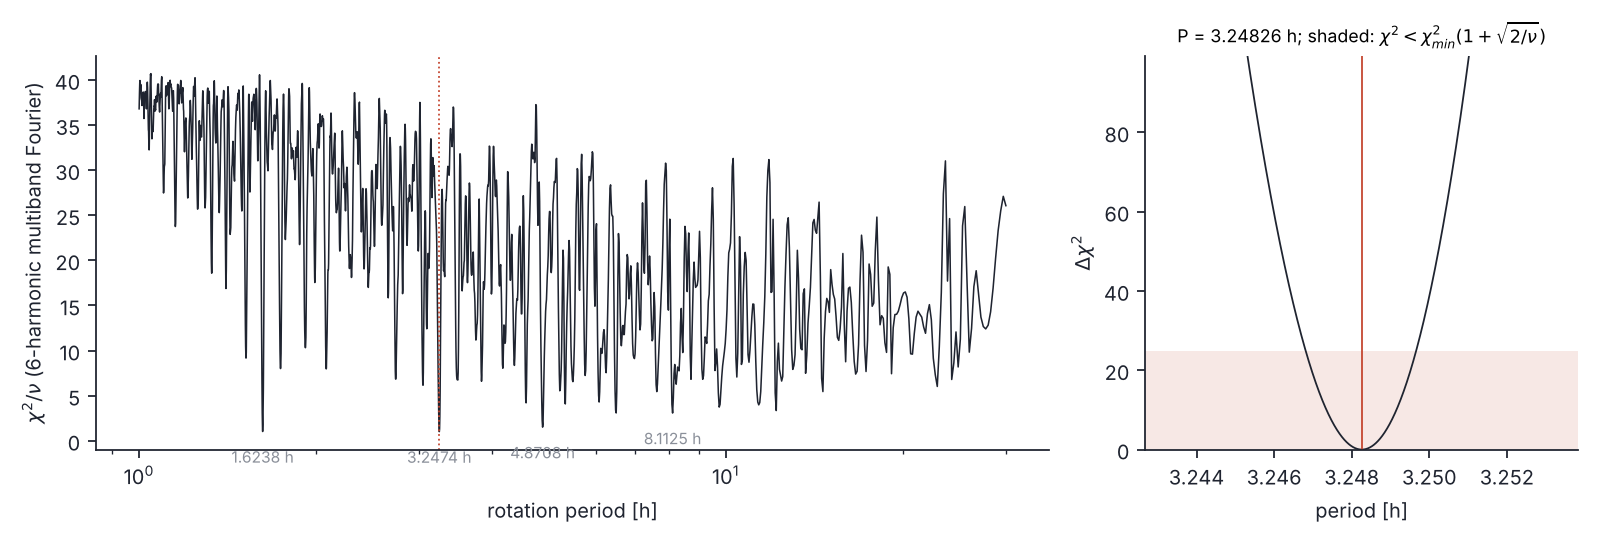
\includegraphics[width=\linewidth]{figures/fig_periodogram.png}
  \caption{Left: multiband six-harmonic Fourier periodogram of 2003~QN$_{21}$. Right: fine scan around
  the adopted period. The shaded band marks $\chi^2<\chi^2_{\min}(1+\sqrt{2/\nu})$.}
  \label{fig:periodogram}
\end{figure}

\begin{table}[t]
\centering
\caption{Model and sampler settings for the 2003~QN$_{21}$ run.}
\label{tab:settings}
\small
\begin{tabular}{@{}>{\raggedright\arraybackslash}p{0.52\linewidth}>{\raggedright\arraybackslash}p{0.44\linewidth}@{}}
\toprule
Quantity & Value\\
\midrule
Facets $N_f$, harmonic degree $l_{\max}$, shape parameters $k$ & 400, 4, 24\\
Lambert weight $c_L$; prior scale $\tau_0$; closure weight $\kappa_{\mathrm{cl}}$ & 0.1; 0.6; 2000\\
Period prior & $\mathcal N(3.24826,\,0.00142^2)$\,h, truncated at $\pm5\sigma$\\
$a/b$ prior & one-sided, $\ge1.337$, $\sigma_{\ln}=0.055$\\
$b/c$ prior & one-sided, $\ge1$, $\sigma_{\ln}=0.05$\\
Jitter prior & log-uniform, 1--100\,mmag\\
Inner optimiser & $K_s=3$, $n_1=40$, $n_2=80$ (L-BFGS)\\
Nested sampling & $n_{\mathrm{live}}=250$, multi-ellipsoid, uniform proposals\\
\bottomrule
\end{tabular}
\end{table}

\subsection{Synthetic test}
An ellipsoid with $a:b:c=1.6:1.1:0.9$, pole $(60^\circ,+50^\circ)$ and $\phi_0=0.7$\,rad was injected
into the same geometry. At the true spin state, the gauge-fixed model reproduces the synthetic data with
$\chi^2=336.9$ for $N=334$. A $20^\circ\times25^\circ$ pole scan peaks at $(80^\circ,+45^\circ)$. The
mirror solution $(260^\circ,-45^\circ)$ lies within 0.2~nats of the peak, and all poles within
0.8~nats of the peak are in the neighbourhoods of the true and mirror poles. This confirms
Proposition~\ref{prop:gauge}, the identifiability of the pole up to the mirror ambiguity, and the
absence of bias at the grid resolution.

\subsection{Nested sampling}
The run used 1955 iterations and $5.87\times10^4$ likelihood evaluations. The acceptance rate dropped
from $\approx28\%$ initially to $\approx3\%$ once the live points occupied the two polar caps. The run
was therefore finalised from its checkpoint at $\Delta\ln Z\approx2.7$ by adding the live points. The
reported $\ln Z=732.2\pm0.25$ (statistical) is consequently approximate. Because the highest
live-point likelihood exceeded the final threshold by only $2.6$~nats, the posterior is adequately
represented. The maximum-likelihood sample has
$(\lambda,\beta,P,\sigma_{\mathrm{jit}})=(145.4^\circ,-78.1^\circ,3.24831\,\mathrm{h},16.5\,\mathrm{mmag})$,
with $\ln\mathcal L=741.26$ and $\chi^2=352.2$ for $N=334$.

\begin{figure}[t]
  \centering
  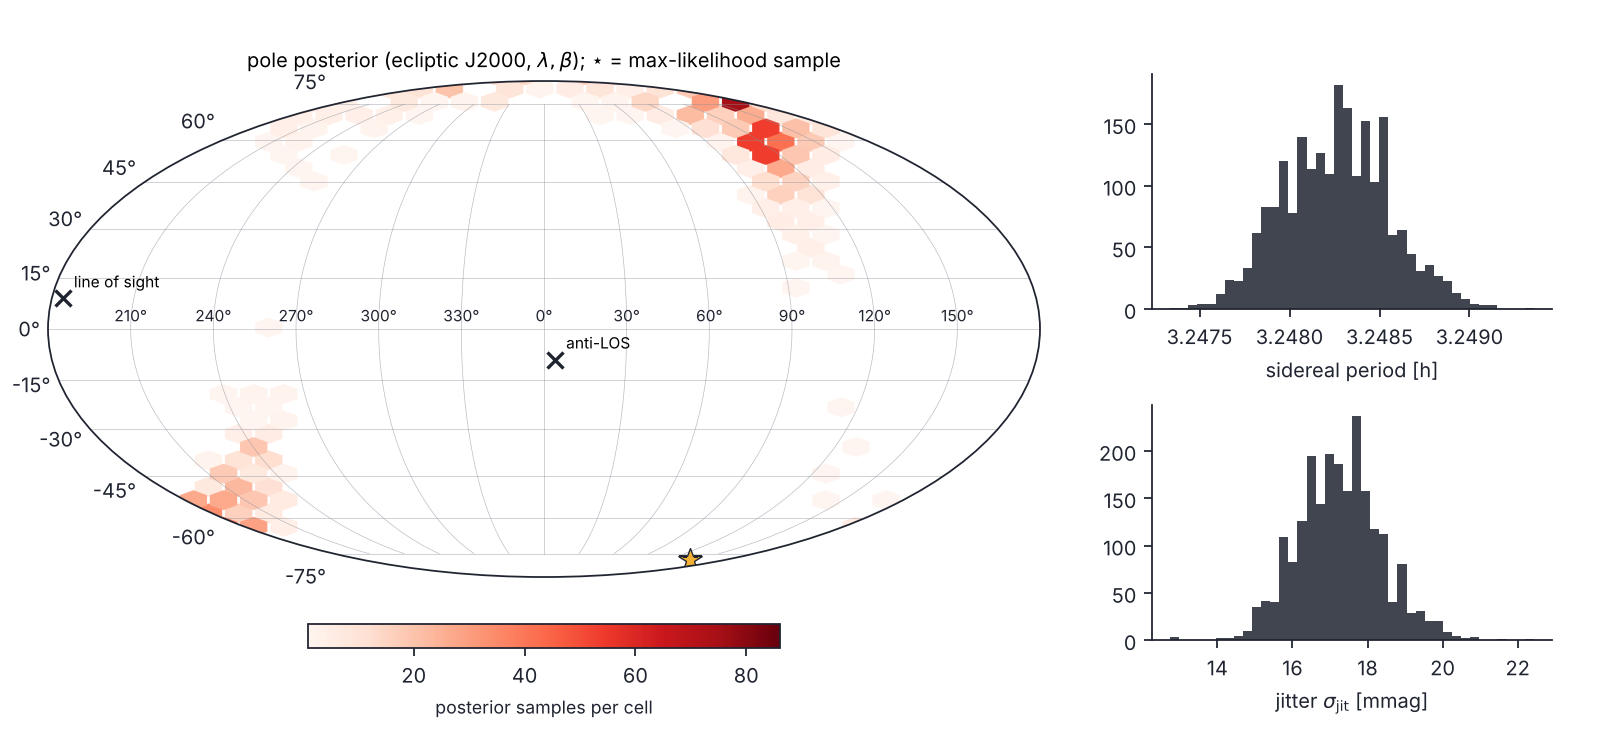
\includegraphics[width=\linewidth]{figures/fig_pole_posterior.png}
  \caption{Posterior of the pole (ecliptic J2000, Mollweide projection), with marginals of the sidereal
  period and the jitter. Crosses mark the line of sight and its antipode; the star marks the
  maximum-likelihood sample.}
  \label{fig:pole}
\end{figure}

\begin{figure}[t]
  \centering
  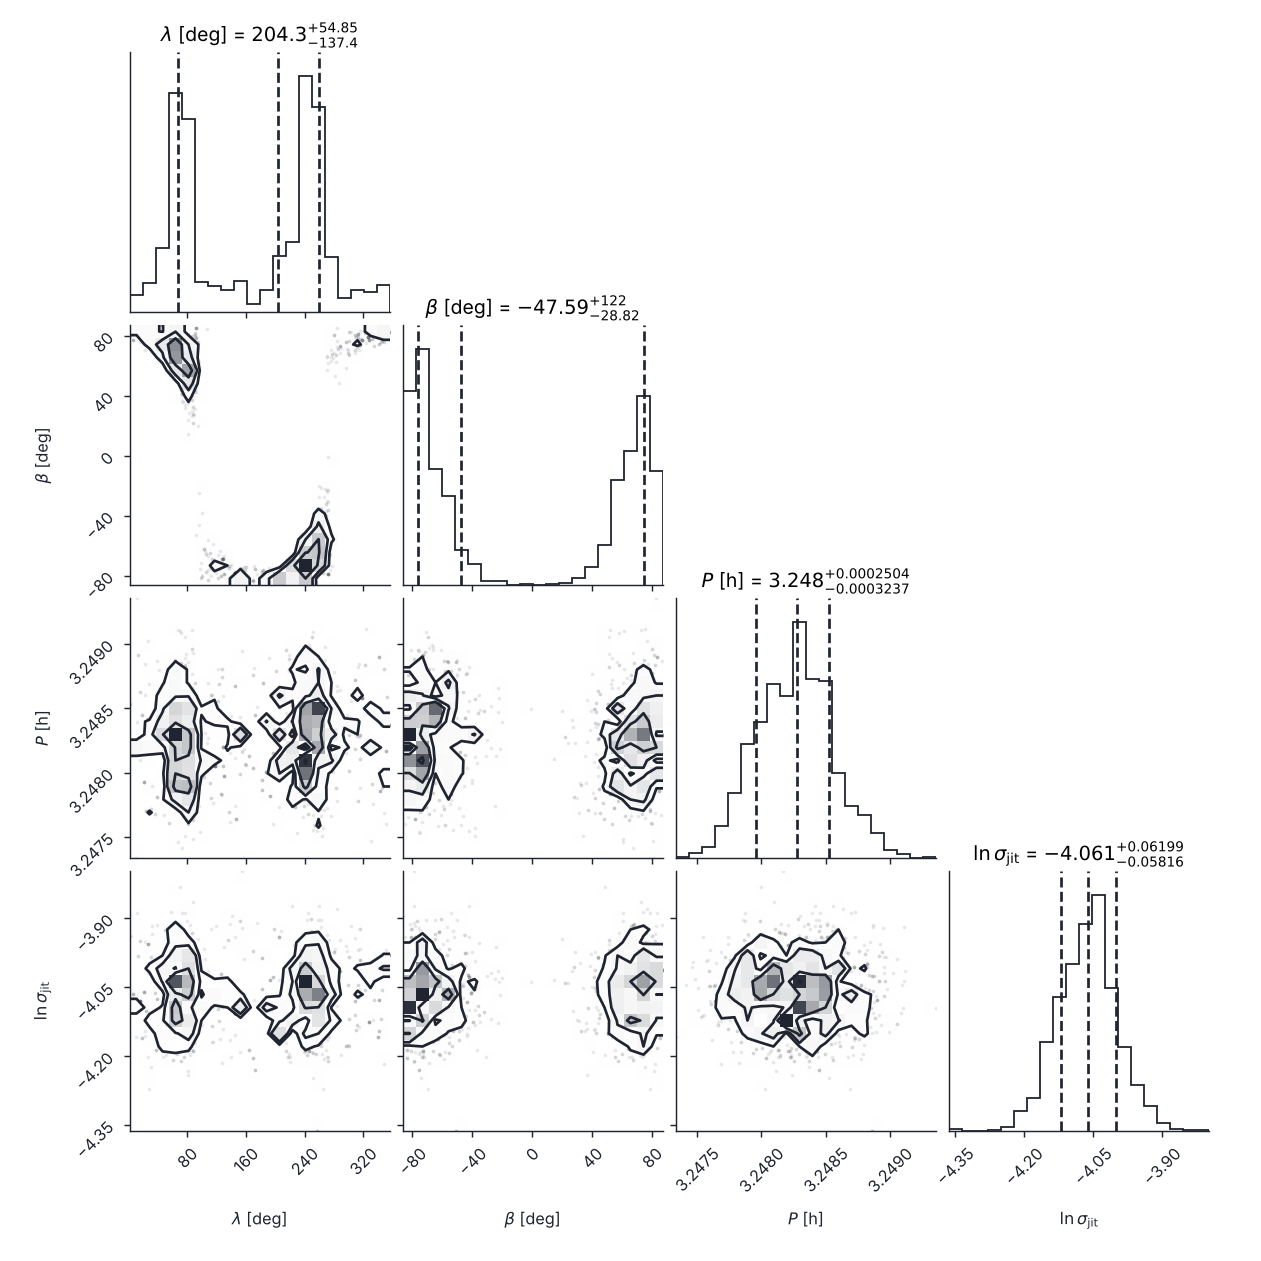
\includegraphics[width=0.78\linewidth]{figures/fig_corner.png}
  \caption{Marginal posteriors of $(\lambda,\beta,P,\ln\sigma_{\mathrm{jit}})$. The quantiles quoted
  for $\lambda$ and $\beta$ are not meaningful summaries of the bimodal distribution; see
  Table~\ref{tab:results}.}
  \label{fig:corner}
\end{figure}

\begin{table}[t]
\centering
\caption{Posterior summaries for 2003~QN$_{21}$. Intervals are 16th--84th percentiles. ``Radius''
denotes the angular radius around the mode's mean pole that encloses the stated posterior mass.}
\label{tab:results}
\small
\begin{tabular}{@{}>{\raggedright\arraybackslash}p{0.36\linewidth}>{\raggedright\arraybackslash}p{0.60\linewidth}@{}}
\toprule
Quantity & Value\\
\midrule
Sidereal period & $3.24828^{+0.00025}_{-0.00032}$\,h\\
Jitter $\sigma_{\mathrm{jit}}$ & $17.2^{+1.1}_{-0.9}$\,mmag\\
Prograde mode & weight 0.47; mean pole $(67^\circ,+71^\circ)$; radius $16^\circ$ (68\%), $34^\circ$ (95\%)\\
Retrograde mode & weight 0.53; mean pole $(244^\circ,-73^\circ)$; radius $15^\circ$ (68\%), $33^\circ$ (95\%)\\
Aspect angle of the line of sight & $86^\circ$--$94^\circ$ (both modes)\\
$\widehat{a/b}$, $\widehat{b/c}$ (projected area) & $1.42\,(1.41$--$1.44)$, $0.87\,(0.84$--$0.91)$\\
Extent ratios $a/b$, $b/c$ (polyhedra) & $1.14\,(1.04$--$1.17)$, $1.10\,(1.01$--$1.17)$\\
Radius uncertainty $\sigma_r$ & median $3.5\%\,\Req$ (range 1.9--5.1\%)\\
Spin axis vs max-inertia axis & $52^\circ$--$88^\circ$ (ensemble), $79^\circ$ (max.\ likelihood)\\
\bottomrule
\end{tabular}
\end{table}

\subsection{Pole, period and noise}
The posterior (Figs.~\ref{fig:pole}, \ref{fig:corner}; Table~\ref{tab:results}) has two modes of
nearly equal weight. They are related by $(\lambda,\beta)\leftrightarrow(\lambda+180^\circ,-\beta)$,
the classical ambiguity of lightcurve inversion for observations near a single plane
\citep{kaasalainen2006}. One apparition cannot break it.

Both modes require an aspect angle close to $90^\circ$. With physically plausible elongations (the
$a/b$ and $b/c$ priors), a 0.40-mag amplitude at $\alpha\approx9^\circ$ is only possible near
equator-on viewing (Proposition~\ref{prop:ab}). The posterior therefore lies along the great circle
perpendicular to the line of sight. Within that circle, the likelihood favours the regions near the
ecliptic poles; the prograde mode extends towards $(\lambda,\beta)\approx(95^\circ,+20^\circ)$. We
cannot determine from these data alone whether this preference is driven by the small phase-angle
signal, by the shape priors, or by both.

The jitter of $17$\,mmag exceeds the median quoted error ($\approx10$\,mmag), indicating systematics
at the 1--2\% level. These include, for example, $i$-band points on nights 1 and 3 that deviate by
$\sim0.05$\,mag from the model (Fig.~\ref{fig:lc}).

\begin{figure}[t]
  \centering
  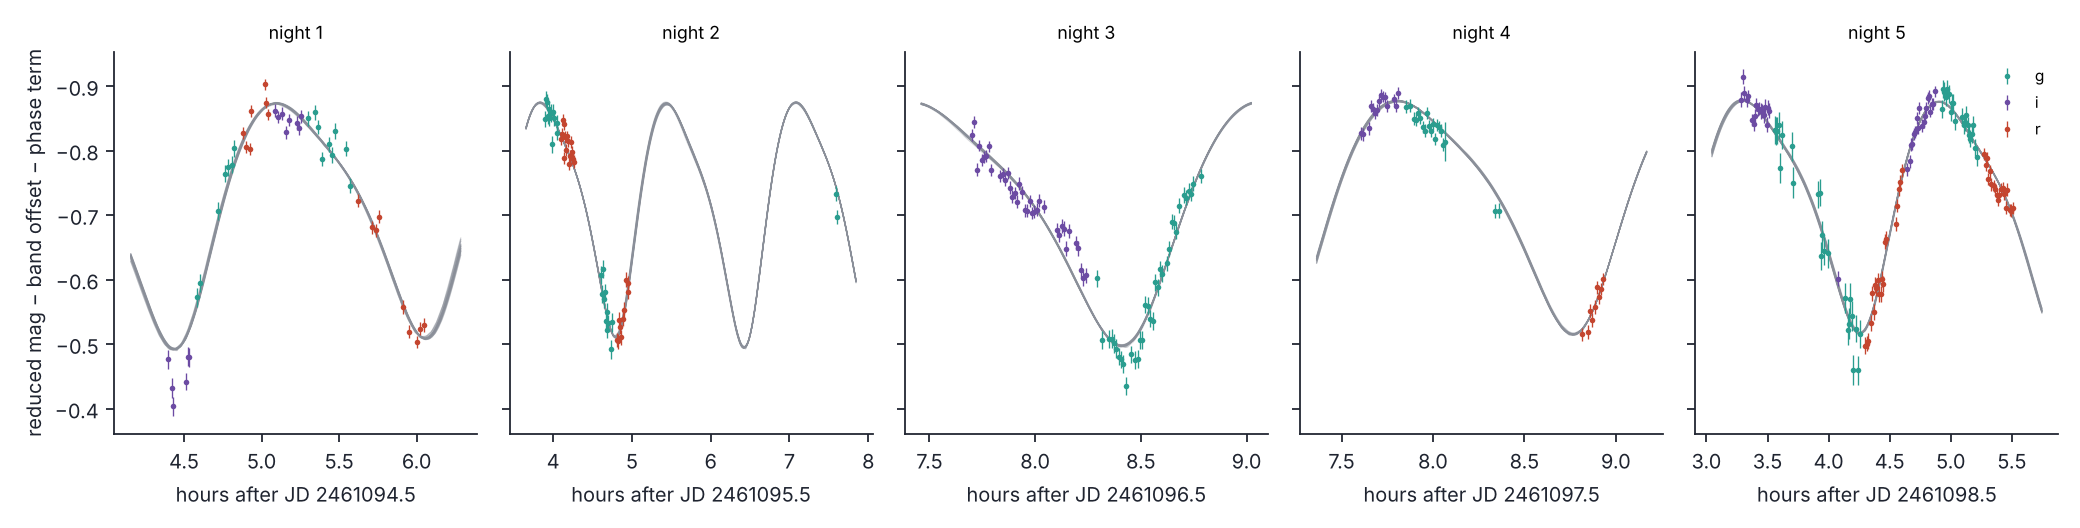
\includegraphics[width=\linewidth]{figures/fig_lightcurves.png}
  \caption{Reduced photometry per night, after subtracting the maximum-likelihood band offsets and phase
  term, with 30 posterior-predictive model curves (grey).}
  \label{fig:lc}
\end{figure}

\subsection{Shape and its uncertainty}
The posterior shapes are box-like rather than ellipsoidal (Fig.~\ref{fig:shapes}). This explains why the
projected-area ratio $\widehat{a/b}=1.42$ substantially exceeds the extent ratio $1.14$. The
radius-uncertainty map is smallest in an equatorial band and largest towards the poles of the body.
This is expected for near equator-on viewing, in which the equatorial silhouette is swept on every
rotation while the polar regions contribute little to the lightcurve (Fig.~\ref{fig:radunc}).

\begin{figure}[t]
  \centering
  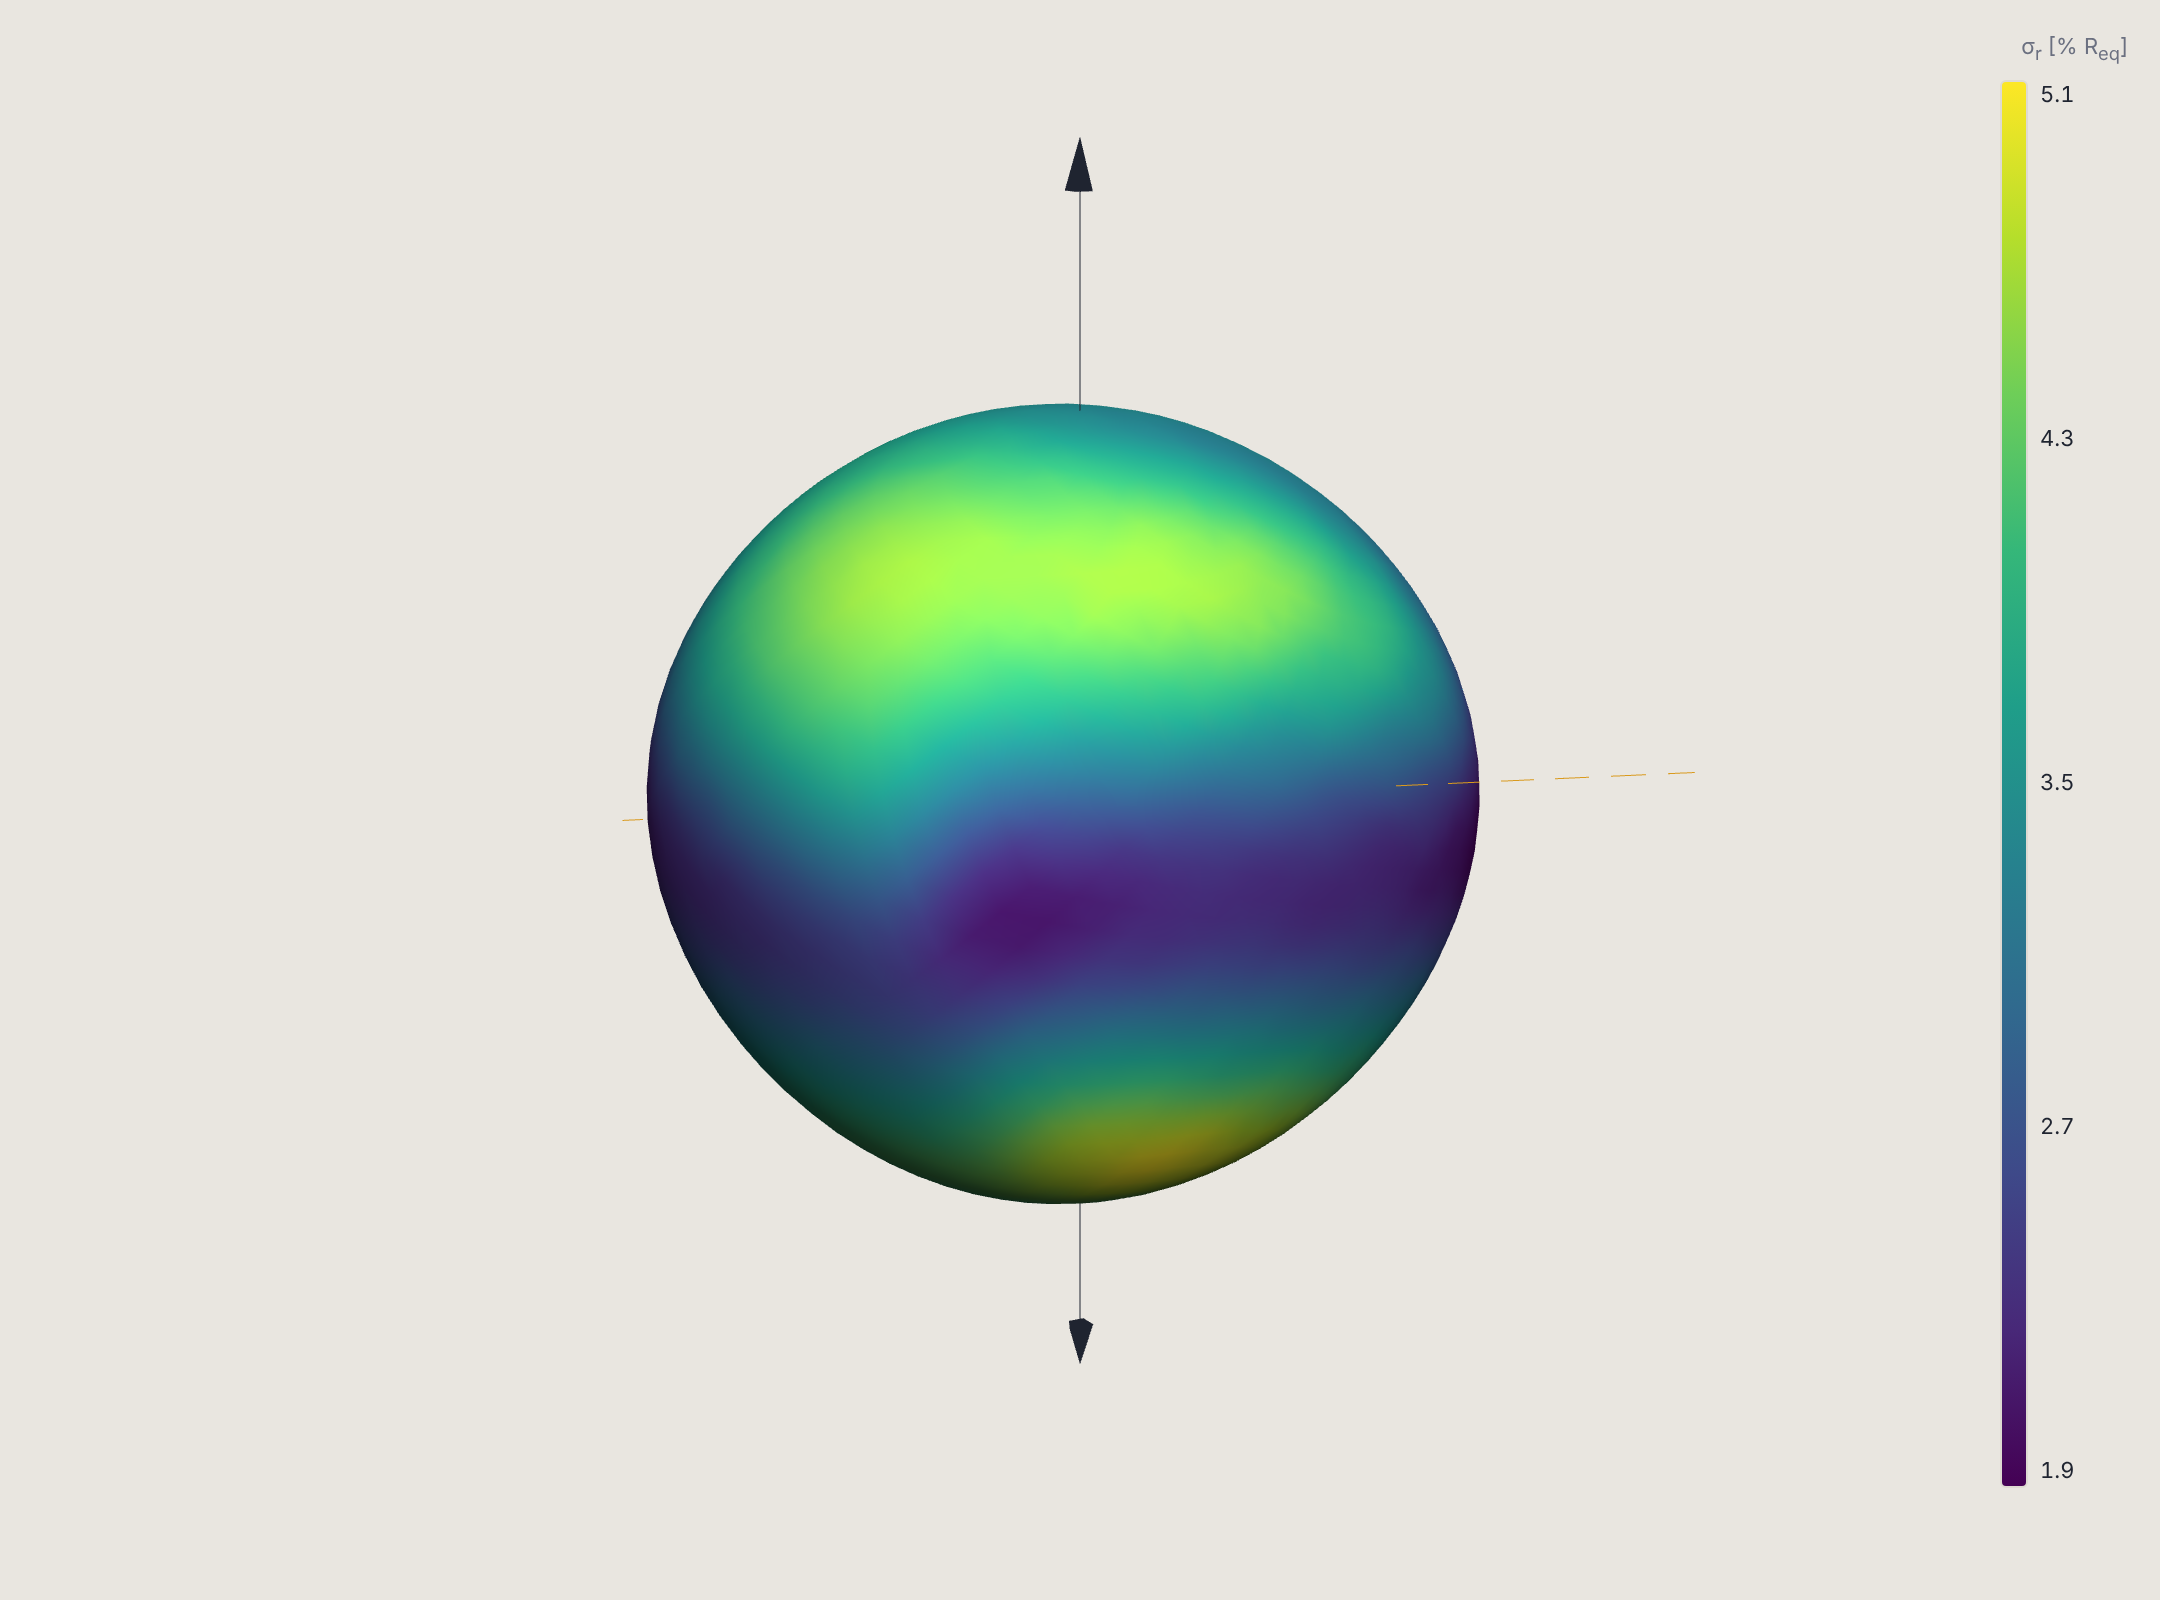
\includegraphics[width=0.72\linewidth]{figures/fig_radius_uncertainty.png}
  \caption{Registered mean shape of 150 posterior draws, coloured by the radius standard deviation
  $\sigma_r$ in per cent of $\Req$ (\S\ref{sec:registration}). The spin axis is vertical; the dashed
  line is the maximum-inertia axis of the mean shape (\S\ref{sec:stability}).}
  \label{fig:radunc}
\end{figure}

\begin{figure}[t]
  \centering
  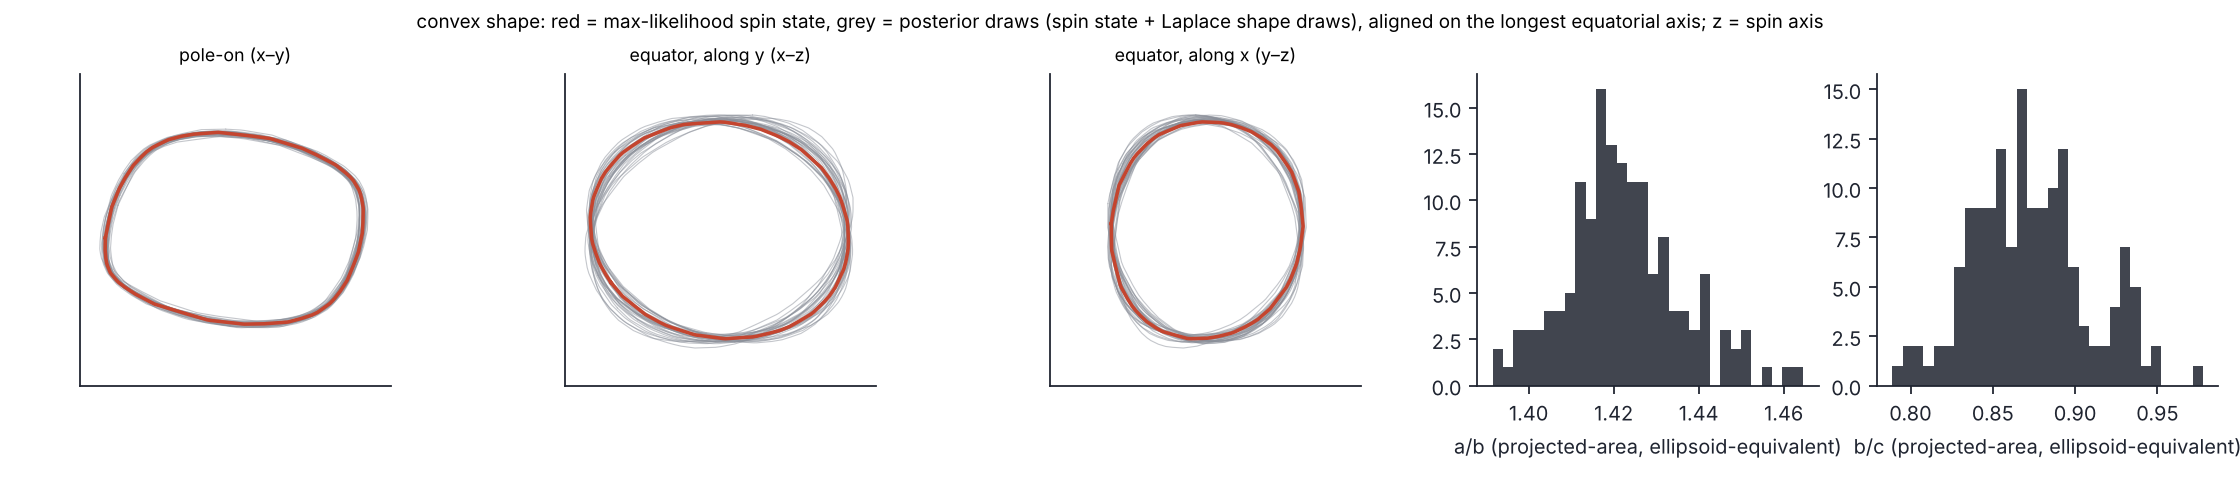
\includegraphics[width=\linewidth]{figures/fig_shapes.png}
  \caption{Silhouettes of the maximum-likelihood shape (red) and posterior draws (grey), registered on
  the longest equatorial axis; $z$ is the spin axis. Right: ellipsoid-equivalent axis ratios
  (Eq.~\ref{eq:ratios}).}
  \label{fig:shapes}
\end{figure}

\subsection{Discretisation}
\label{sec:resolutionresult}
Re-weighting 300 posterior samples from $N_f=400$ to $N_f'=800$ gives an ESS fraction of 0.79, with a
standard deviation of $\ln\mathcal L$ differences of 0.93~nats. The prograde fraction changes from
0.443 to 0.445, and the mean poles move by $<1.3^\circ$ (to $(66.9^\circ,+69.1^\circ)$ and
$(242.2^\circ,-73.7^\circ)$). The facet discretisation is therefore not a limiting factor.

\subsection{Rotational stability}
The stability diagnostic (\S\ref{sec:stability}) is negative. The maximum-likelihood shape has
normalised principal moments $0.73:0.92:1.00$, with the maximum-inertia axis $79^\circ$ from the spin
axis. Across the ensemble the angle ranges from $52^\circ$ to $88^\circ$, and it is $77^\circ$ for the
registered mean shape. The soft constraint $\widehat{b/c}\ge1$ was overridden by the data (posterior
$\widehat{b/c}=0.87$). Being a projected-area proxy, it does not constrain the inertia tensor in any
case. These shapes are therefore not physically admissible relaxed rotators. The pole and shape results
above should be regarded as provisional until the inversion is repeated with a constraint on the
inertia tensor (\S\ref{sec:discussion}).

%==========================================================================================
\section{Discussion and outlook}
\label{sec:discussion}

\paragraph{Physical admissibility.} The most important improvement is to impose principal-axis
rotation directly. For a Gaussian image, the inertia tensor of the reconstructed body is not an
explicit function of $\vect c$, because it requires the support distances $\vect h$. Practical options
include:
\begin{itemize}[nosep]
\item a differentiable inner Minkowski step, with a penalty on the off-diagonal elements of
  $\mathsf I$ and on $I_{zz}<\max(I_{xx},I_{yy})$;
\item a support-function parametrisation of the shape, in which the volume and inertia integrals are
  explicit;
\item rejection of posterior samples by the diagnostic of \S\ref{sec:stability}, which is less
  efficient.
\end{itemize}

\paragraph{Geometry diversity.} A single apparition spanning $\sim1.3^\circ$ in phase angle constrains
the pole only through the amplitude--aspect relation. Combining the dense lightcurves with sparse survey
photometry from other apparitions is straightforward in this framework, because each subset simply
contributes its own geometry and band offsets \citep{durech2009}. That combination will resolve the
mirror ambiguity and shrink the modes.

\paragraph{Approximations.} The Laplace approximation is local. If the conditional shape posterior is
multimodal or strongly non-Gaussian, $\ln\mathcal L(\vect\theta)$ is biased. Full Hamiltonian Monte
Carlo over $(\vect\theta,\vect c)$, e.g.\ with NUTS \citep{hoffman2014} on the differentiable model,
would test this at selected spin states, in the spirit of \citet{muinonen2020}. The scattering law and
the linear phase term are adequate for a short arc. Wider phase coverage requires a proper phase
function and, possibly, a free Lambert weight.

\paragraph{Sampling.} The polar-cap inefficiency (Remark in \S\ref{sec:nested}) can be removed by a
singularity-free pole parametrisation. Alternatively, slice-based proposals can be used, or the
four-dimensional posterior can be sampled with dynamic nested sampling targeted at posterior mass.

%==========================================================================================
\section*{Data and code availability}
The \texttt{lcinv} prototype implements all steps described here: ephemerides, period search, the JAX
likelihood, nested sampling, Minkowski reconstruction, the radius-uncertainty maps and the diagnostics.
It also includes the validation scripts, the cached Horizons vectors and the outputs for
2003~QN$_{21}$. The implementation relies on JAX \citep{jax2018}, Optax \citep{optax2020},
\texttt{dynesty} \citep{speagle2020}, Astropy \citep{astropy2022}, \texttt{astroquery}
\citep{ginsburg2019} and Qhull \citep{barber1996}.

\bibliographystyle{plainnat}
\bibliography{references}

%==========================================================================================
\appendix
\section{Notation}
\begin{tabular}{@{}ll@{}}
\toprule
Symbol & Meaning\\
\midrule
$y_i$, $e_i$, $\sigma_i$ & reduced magnitude, quoted error, total error (Eq.~\ref{eq:jitter})\\
$\uv s_i$, $\uv e_i$, $\alpha_i$ & asteroid$\to$Sun and asteroid$\to$observer directions, phase angle\\
$(\lambda,\beta)$, $P$, $\phi_0$ & ecliptic pole, sidereal period, rotational phase at $t_{\mathrm{ref}}$\\
$\uv n_j$, $A_j$, $N_f$ & facet normals, facet areas, number of facets\\
$c_{lm}$, $k$, $\tau_l$ & harmonic shape coefficients, their number, prior scales\\
$\vect\eta=(o_b,s)$ & band offsets and phase slope (profiled)\\
$\mathcal L(\vect\theta)$ & Laplace-marginalised likelihood of the spin state (Eq.~\ref{eq:laplace})\\
$h_j$, $F_j$, $V$ & support distances, realised facet areas, volume (Minkowski step)\\
$r(\uv u)$, $\Req$ & radial function, volume-equivalent radius\\
\bottomrule
\end{tabular}

\section{Algorithm summary}
\begin{enumerate}[leftmargin=*]
\item Read the photometry, query Horizons and compute light-time-corrected $\uv s_i$, $\uv e_i$,
  $\alpha_i$ and reduced magnitudes (\S\ref{sec:geometry}).
\item Compute the multiband Fourier periodogram; obtain $P_0$, its intervals, the amplitude, $A(0)$ and
  the $a/b$ bound (\S\ref{sec:period}).
\item For each spin state proposed by the nested sampler:
  \begin{enumerate}[nosep]
  \item build $\mathsf S(\vect\theta)$ (Eq.~\ref{eq:brightness}) with $\phi_0=0$;
  \item run the coarse-to-fine L-BFGS minimisation of $f(\vect c)$, profiling $\vect\eta$ at every
    evaluation;
  \item return $\ln\mathcal L(\vect\theta)$ from Eq.~\eqref{eq:laplace}.
  \end{enumerate}
\item Resample the nested-sampling output to equal weights.
\item For a subset of the samples, draw $\vect c\sim\mathcal N(\hat{\vect c},\mathsf H^{-1})$, solve the
  Minkowski problem (Eq.~\ref{eq:minkowski}), register the shapes about $z$ and compute
  radius-uncertainty maps and inertia diagnostics.
\item Re-weight with a finer facet grid to verify discretisation convergence.
\end{enumerate}

\end{document}
